\begin{figure}[tb]
    \centering % avoid the use of \begin{center}...\end{center} and use \centering instead (more compact)
    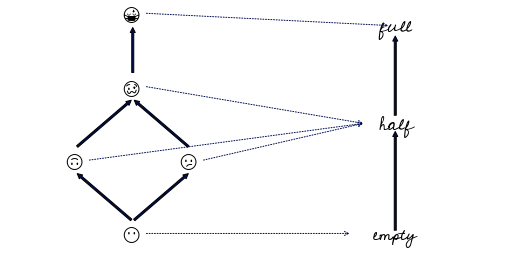
\includegraphics[width=\columnwidth]{monoid_maps.png}
    \caption{Monoids support partial ordering, such as the two emojis with tilted mouths being at the same rank above and below emojis with different mouth positions. The monotonic map on the right is a meta ordering of the partial order.  Figure inspired by definition 1.59 diagram in Spivak and Fong's An Invitation to Applied Category Theory \cite{fongInvitationAppliedCategory2019}}
    \label{fig:data_partial_order}
  \end{figure}
  




  Expressiveness, as defined by Mackinlay \cite{mackinlayAUTOMATICDESIGNGRAPHICAL1987, mackinlayAutomatingDesignGraphical1986} is a measure of how much of the structure any map can encode. A fully expressive component is one that is equivariant since it has preserved all the structure in the data. Models of visualization evaluate this equivariance and how elements built in the model can be composed to build more complex visualizations. Mackinlay's \textit{A Presentation Tool} (APT) introduced the notion of visualizations having syntax and semantics \cite{mackinlayAutomatingDesignGraphical1986} and Wilkenson described the grammar of this language \cite{wilkinsonGrammarGraphics2005}. This grammar oriented approach allows users to describe how to compose visual elements into a graphical design \cite{wongsuphasawatNavigatingWideWorld2021}, while we are proposing a framework for building those elements. 
  

  
  
  